\begin{figure}[ht]
    \begin{subfigure}[t]{0.7\textwidth}
        \caption{}
        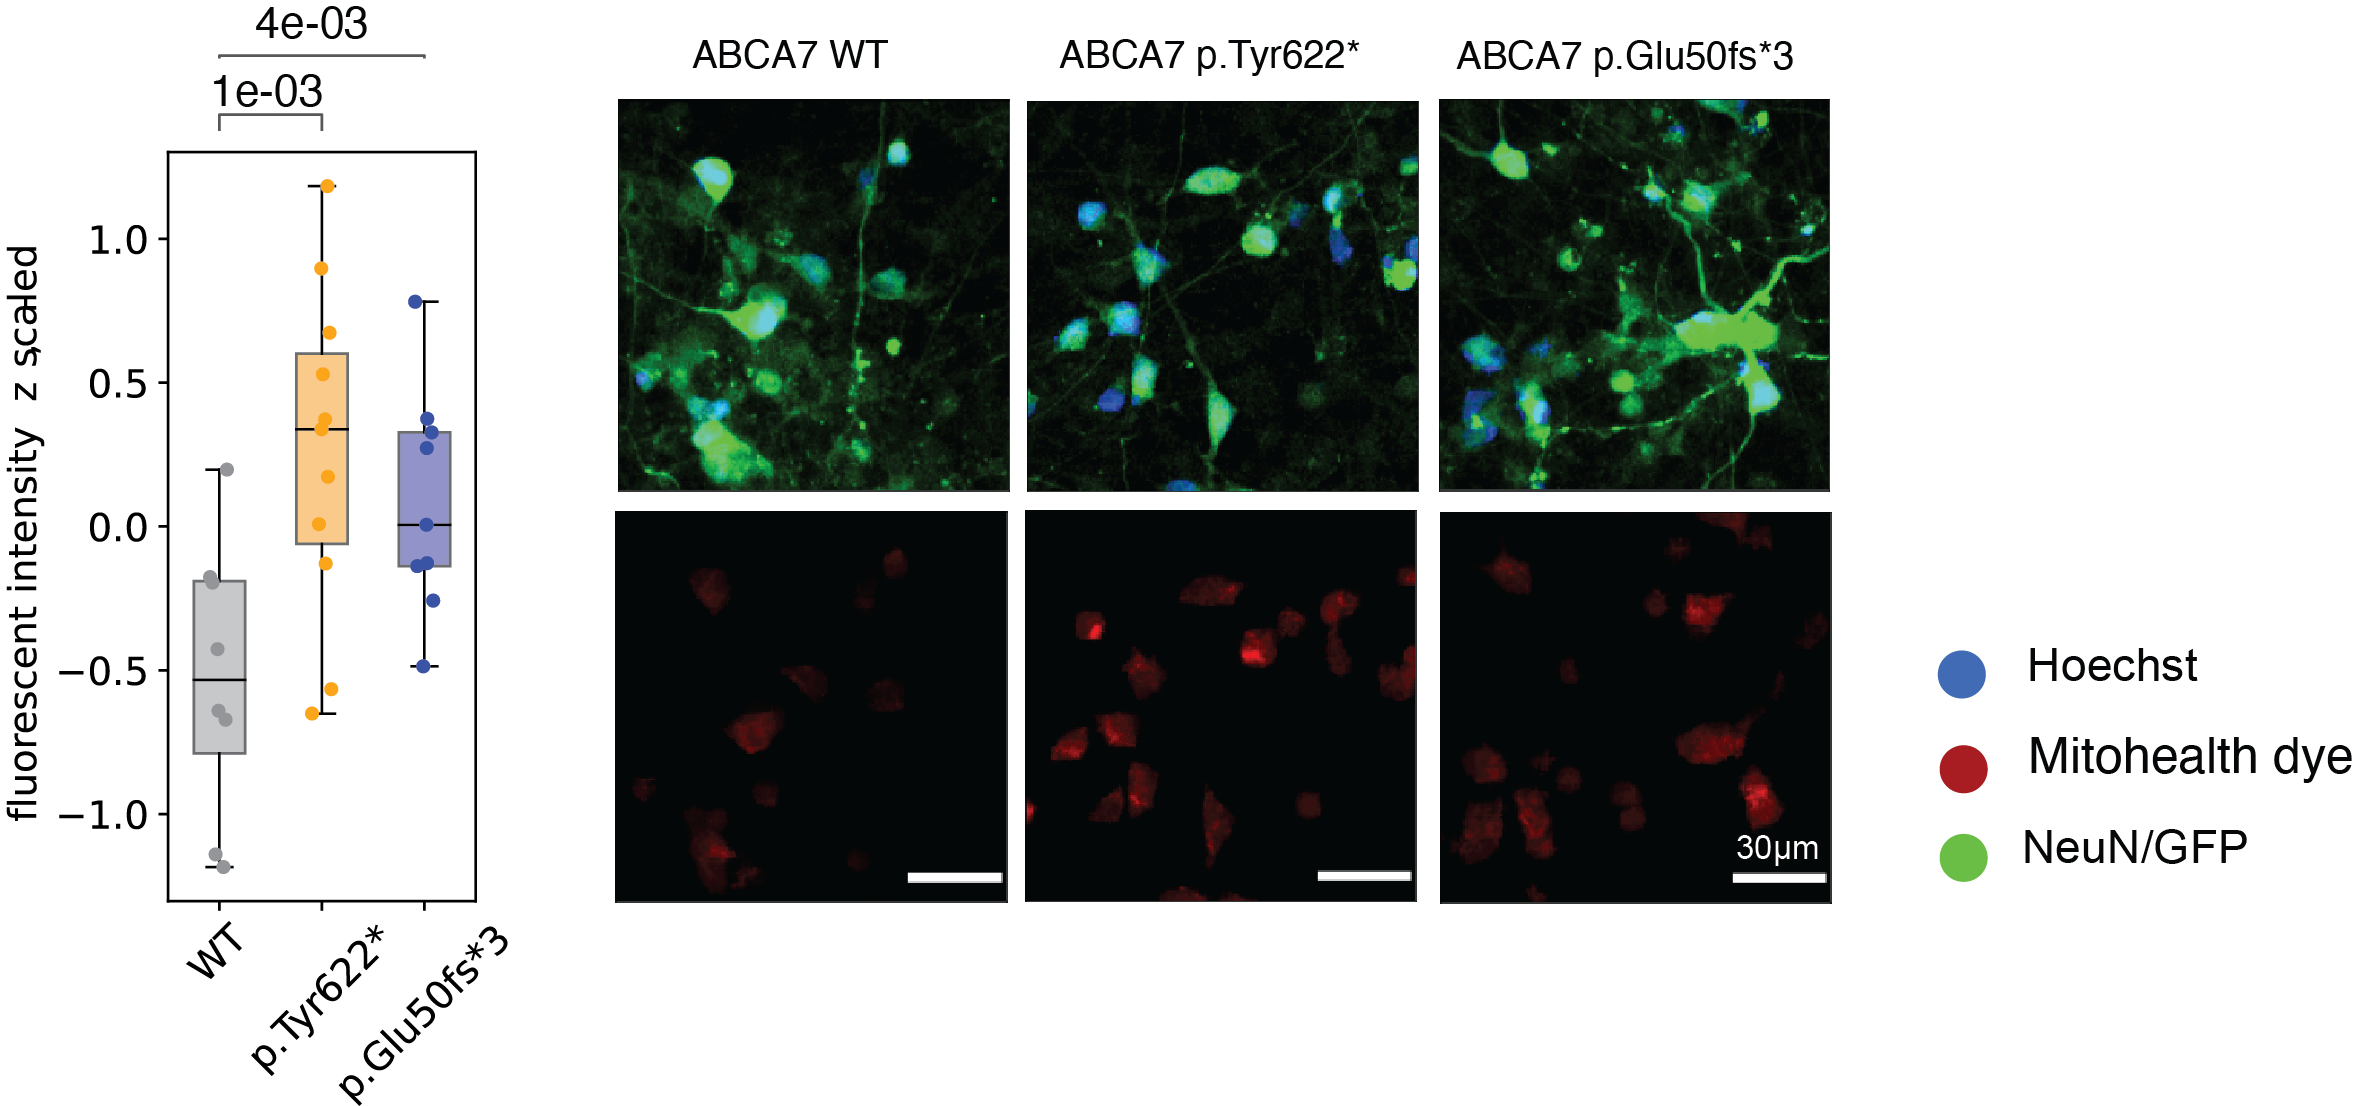
\includegraphics[width=\textwidth]{./extended_plots/mitohealth_dye.png}        
    \end{subfigure}
    \par
    \begin{subfigure}[t]{\textwidth}
        \caption{}
        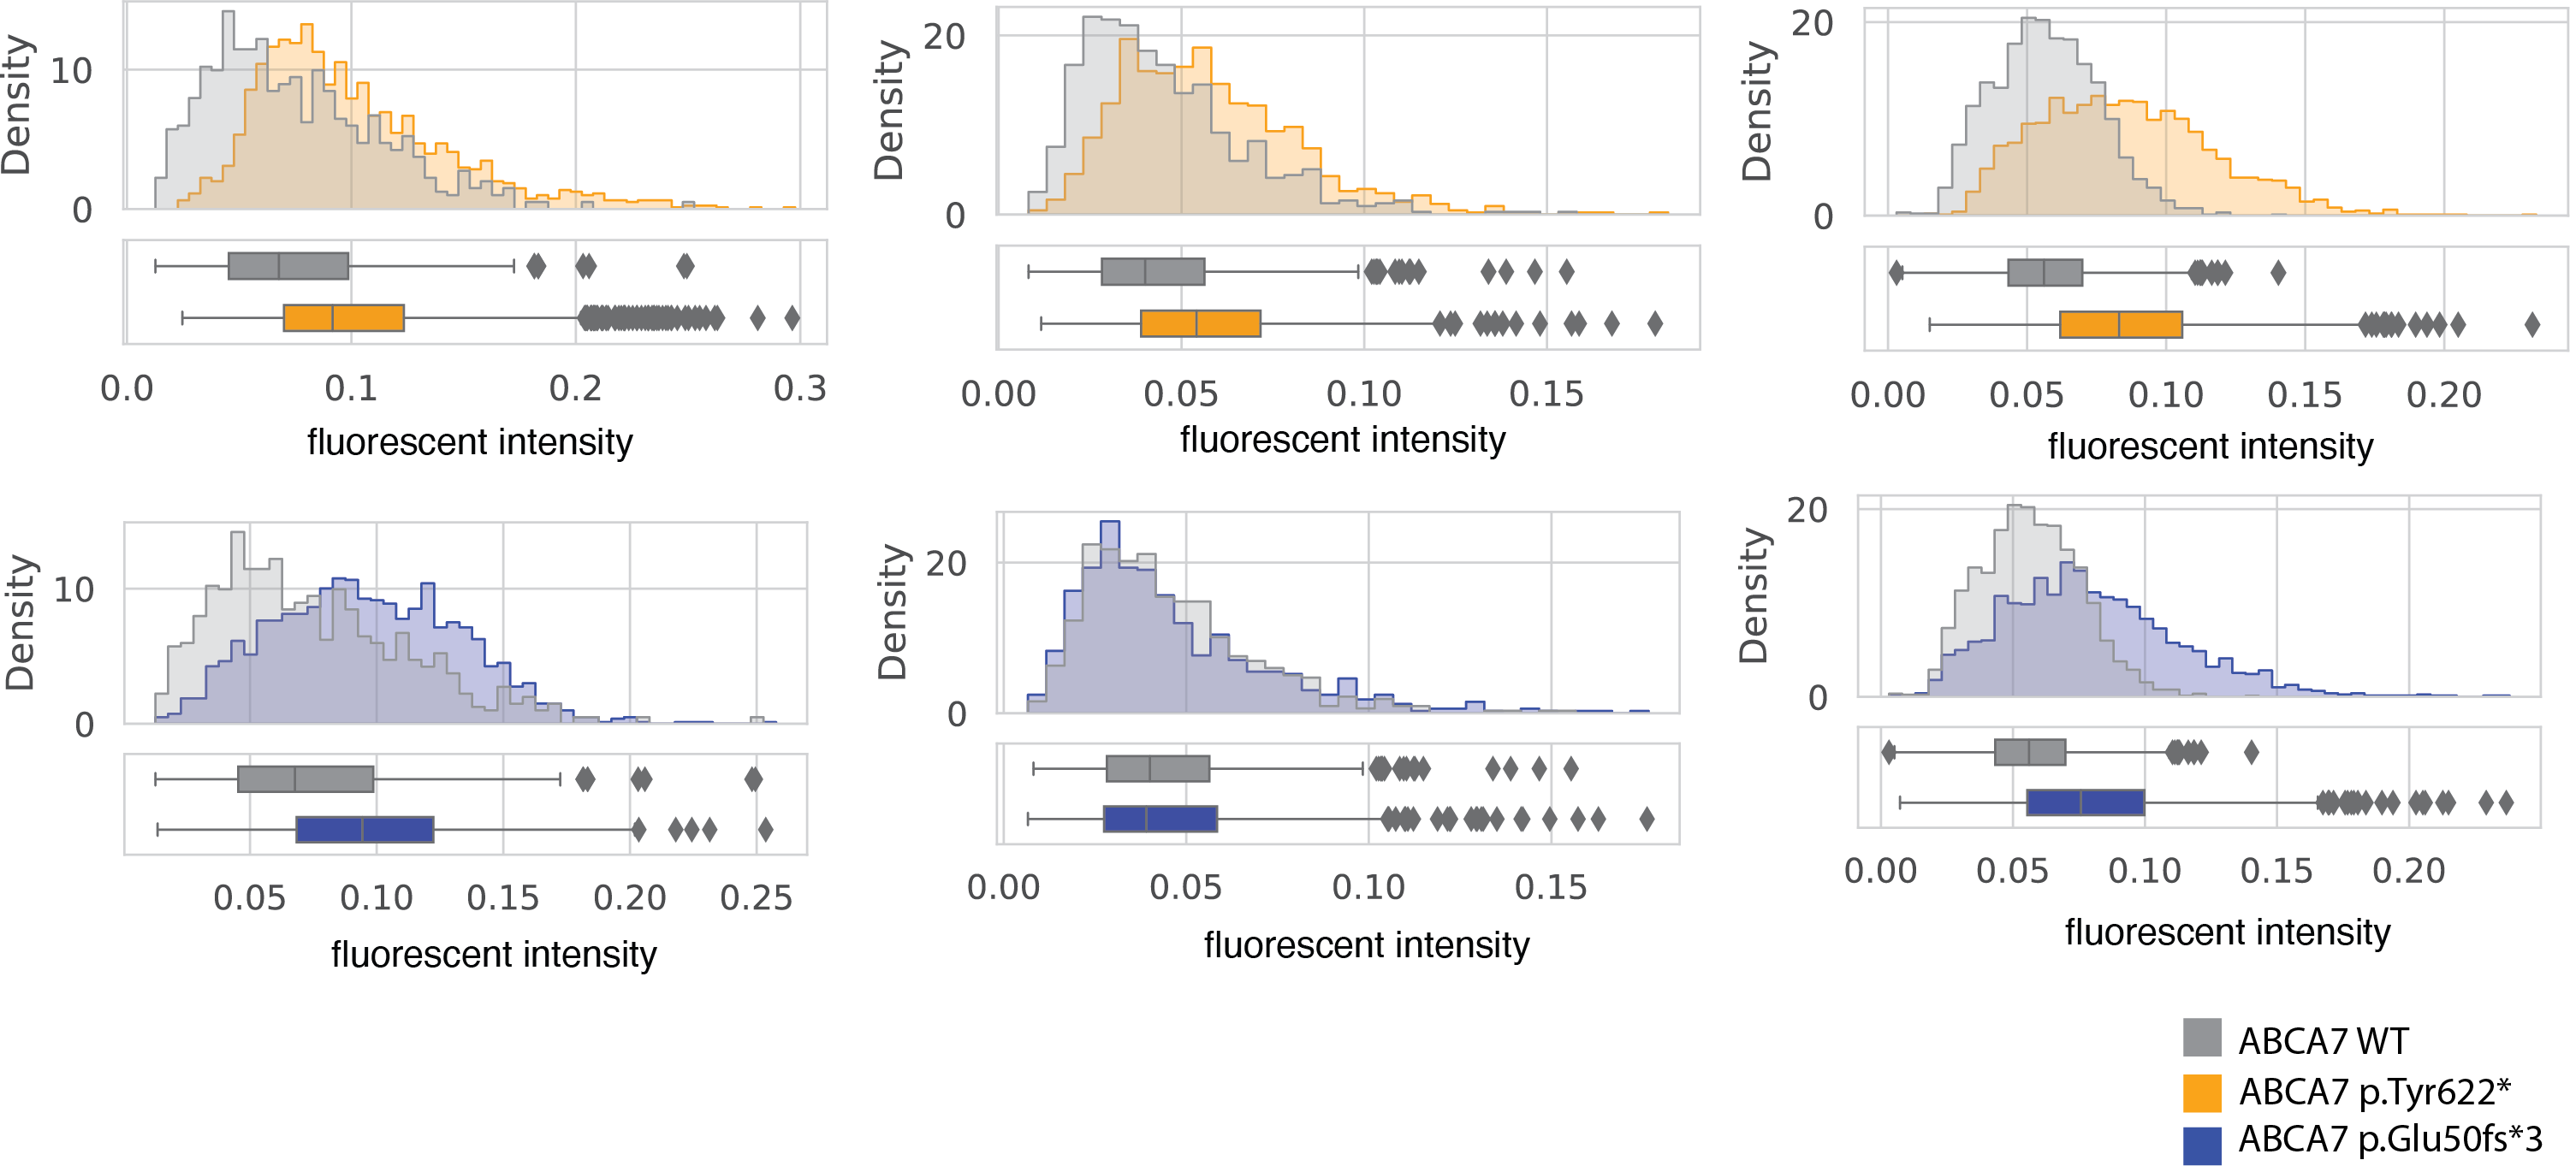
\includegraphics[width=\textwidth]{./extended_plots/mitohealth_per_cell.png}        
    \end{subfigure}
    \caption{
         \textbf{Analysis of Oxygen Consumption Rates in ABCA7 LoF vs. Control iNs.}\\[1ex]
         (A) Example oxygen consumption rate (OCR) curves from Batch 1 of the two differentiation batches used for analysis in Figure~\ref{fig:main_mitochondrial}G. The line plot indicates the per-condition mean estimator, and the error bars indicate the 95\% confidence interval. 
         (B) Representative per-well traces from (A). 
         (C) Schematic indicating measurement of maximal and basal oxygen consumption to compute SRC, as shown in 
         (D) for WT, ABCA7 p.Glu50fs*3, and ABCA7 p.Tyr622* iNs. P-values computed by independent sample t-test. $N$ wells = 18 (WT), 17 (p.Tyr622*), 13 (p.Glu50fs*3) across two independent differentiation batches and Seahorse experiments. 
         (E) Relative uncoupling measured for two independent iN differentiation batches and separate Seahorse experiments shown combined in Figure~\ref{fig:main_mitochondrial}G. P-values computed by independent sample t-test. Batch 1 (left); $N$ wells = 10 (WT), 7 (p.Tyr622*), 7 (p.Glu50fs*3). Batch 2 (right); $N$ wells = 8 (WT), 10 (p.Tyr622*), 6 (p.Glu50fs*3) shown per differentiation batch. For (D, E) boxes indicate per-condition dataset quartiles, and whiskers extend to the most extreme data points not considered outliers (i.e., within 1.5 times the interquartile range from the first or third quartile). 
         (F) Per-batch cell-level MioHealth fluorescence intensities (related to Figure~\ref{fig:main_mitochondrial}H).
     }
     \label{fig:oxygen_consumption_rates_iPSC_neurons}
 \end{figure}